\documentclass[../../main/main.tex]{subfiles}
\begin{document}
\section{Nash Equilibrium Strategy Profile}


The full solution process is detailed in Appendix \ref{app:derivation}. Here we present the final solution, which was obtained by solving for $c(s)$ in terms of $x_2$, then using this to solve for $v(s)$, and finally solving for $b(s)$ up to a constant of integration. The resulting system of 7 equations in 7 unknowns was solved symbolically using Mathematica and simplified by finding common subexpressions $A_0, A_1, A_2, A_3, A_4, A_5$. 

\begin{theorem}[Nash Equilibrium Strategy Profile]
    \label{thm:nash_equilibrium}
The unique admissible Nash equilibrium strategy profile for Limit Continuous Poker with minimum bet size $L$ and maximum bet size $U$ is given by:

\begin{align*}
    x_0 &= \frac{3 (L+1)^3 U}{A_4}\\
    x_1 &= \frac{3 A_0 L U+A_0 U-L^3-3 L^2}{A_4}\\
    x_2 &= \frac{A_5}{A_4}\\
    x_3 &= \frac{A_2 L^3+3 A_2 L^2+3 L \left(5 U^3+15 U^2+15 U+4\right)+4 U^3+12 U^2+12 U+3}{A_4}\\
    x_4 &= \frac{3 A_1 L^2+A_2 L^3+3 A_2 L+4 U^3+12 U^2+12 U+3}{A_4}\\
    x_5 &= \frac{3 A_3 L^2+3 A_3 L+A_3+L^3 \left(6 U^3+18 U^2+15 U+2\right)}{A_4}\\
    b_0 &= -\frac{(L+1)^3}{\text{A4}} \\ 
    b(s) &= b_0 - \frac{(1+3s)(x_2-1)}{6(1+s)^3}\\
    c(s) &= \frac{x_2+s}{s+1}\\
    v(s) &= \frac{x_2+2 s^2+4 s+1}{2 (s+1)^2}
\end{align*}

where the common subexpressions are:

\begin{align*}
	A_0 &= U^2+3 U+3 \\
    A_1 &= 7 U^3+21 U^2+21 U+6 \\
    A_2 &= 6 U^3+18 U^2+18 U+5 \\
    A_3 &= 7 U^3+21 U^2+18 U+3 \\
    A_4 &= 3 A_1 L^2+3 A_1 L+A_1+A_2 L^3 \\
    A_5 &= 3 A_0 L^2 U+3 A_0 L U+A_0 U-L^3
\end{align*}
\end{theorem}

Proof given in Appendix \ref{app:derivation}. Refer to section \ref{subsec:nash_equilibrium_structure} for an explanation of how these values fit together to actually form the strategy profile.

This solution is more interpretable in graphical form. Figure \ref{fig:strategyprofile} shows the strategy profile for various values of $L$ and $U$ ranging from very lenient ($L=0, U=10$) to very restricted ($L=0.5, U=1$). The more lenient bet size limits model something closer to NLCP, while the more restricted bet size limits model something closer FBCP with a fixed bet size. Indeed, we see that the strategy profile of for $L=0, U=10$ looks qualitatively similar to the strategy profile of NLCP - we will show in section \ref{sec:strategic_convergence} that the strategy profile approaches the Nash equilibrium of NLCP as $L$ and $U$ approach $0$ and $\infty$, respectively, and that the strategy profile approaches the Nash equilibrium of FBCP as $L$ and $U$ approach some fixed value $s$ from either side.

\begin{figure}[h!]
    \begin{adjustwidth}{-1in}{-1in}
        \centering
        \begin{minipage}{0.6\textwidth}
            \centering
            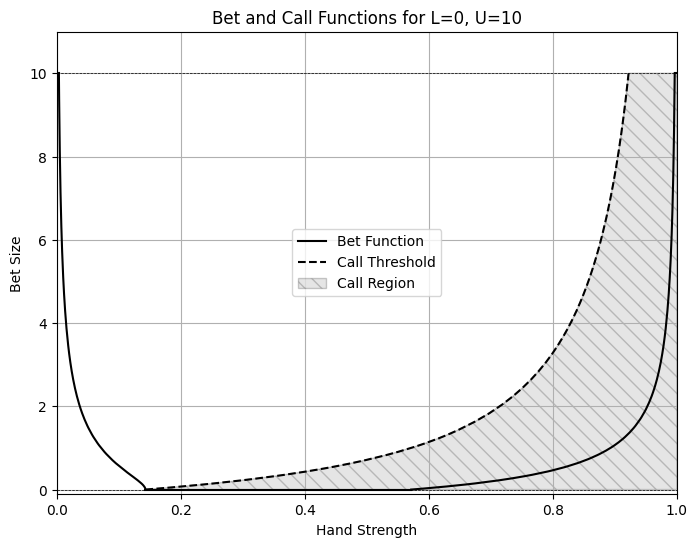
\includegraphics[width=\textwidth]{images/limit_continuous_0_10.png}
        \end{minipage}
        \hspace{0.05\textwidth}
        \begin{minipage}{0.6\textwidth}
            \centering
            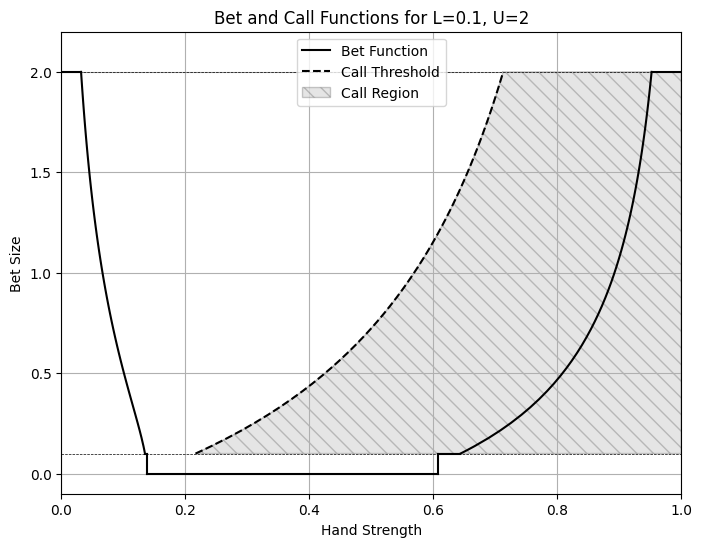
\includegraphics[width=\textwidth]{images/limit_continuous_0.1_2.png}
        \end{minipage}
        \vspace{0.5cm}\\
        \begin{minipage}{0.6\textwidth}
            \centering
            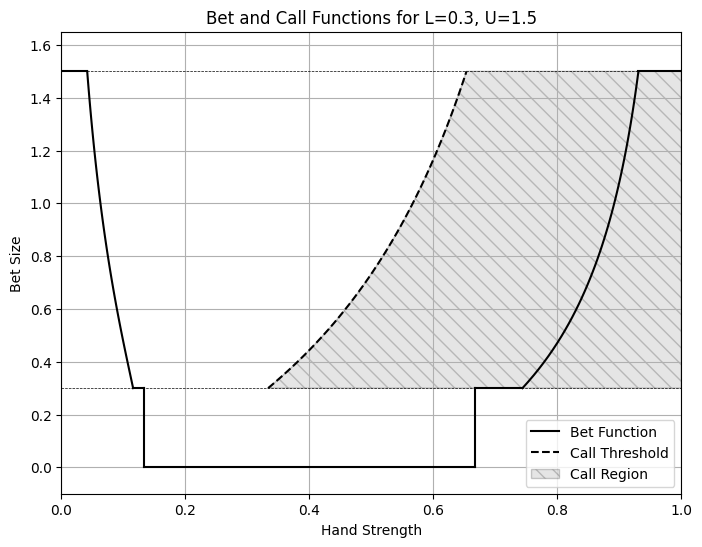
\includegraphics[width=\textwidth]{images/limit_continuous_0.3_1.5.png}
        \end{minipage}
        \hspace{0.05\textwidth}
        \begin{minipage}{0.6\textwidth}
            \centering
            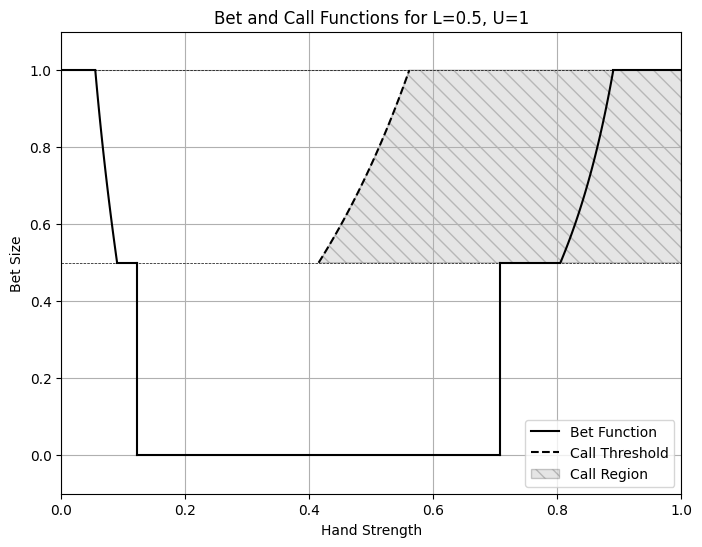
\includegraphics[width=\textwidth]{images/limit_continuous_0.5_1.png}
        \end{minipage}
    \end{adjustwidth}
    \caption{Nash equilibrium strategy profiles for different values of $L$ and $U$, from very lenient to very restricted bet sizes. The bet function maps hand strengths to bet sizes, while the call function gives the minimum calling hand strength for a given bet size. The shaded regions represent the hand strengths for which the caller should call a given bet size.}
    \label{fig:strategyprofile}
\end{figure}


\end{document}
